\section{Experiments}

\subsection{Z-score Versus Activation-score}

Z-score is one of the most used methods in linguistic statistics. It compares the observed frequency of a word with the frequency expected in case of a "normal" distribution. This calcul gives easily for example the most specific vocabulary of a given author in a contrastive corpora. The highest z-score are the most specific word in this case. This is a simple but strong method to analyze feature on text. It can be also used to classify word sequences according to the global z-score (sum of the score) in the sequence. The mean accuracy of this methods on our data set is around 85\%, that confirm z-score is really meaningful on contrastive data. On the other hand, the deep learning reaches most of time more than 90\% on text classification. It means the training methods can learn also by themselves some sort of linguistic specificities useful to distinguish class of text or authors. We've seen on image that's the role of the convolution. It learns an abstraction on the data to make classification easier. The question is : what is the nature of this abstraction on text ? We going to seen now that the deep learning detect automatically words with hight z-score but apparently it's not this only linguistic marks detected.

\begin{figure}[h]
\begin{center}
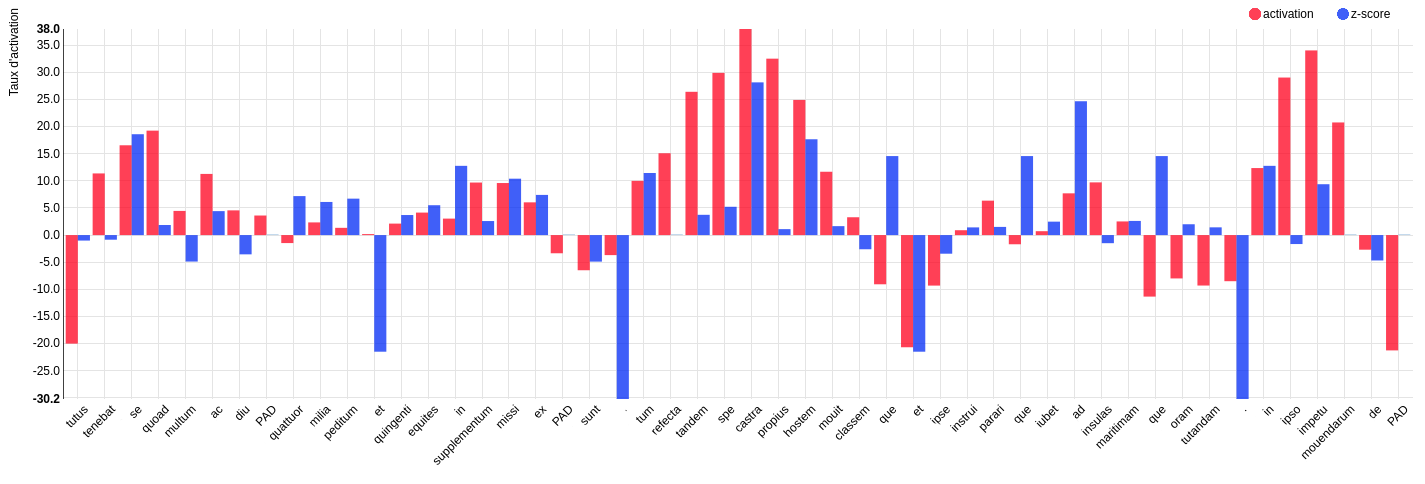
\includegraphics[width=16cm]{img/z-score_activations.png}
\caption{Latin dataset : Livy Book XXIII Chap. 26 - Z-score Vs Activation-score}
\label{comparision}
\end{center}
\end{figure}

The Figure \ref{comparision} shows us a comparison between z-score and activation-score on a sequence extract form our latin corpora. Here it's an example where Livy\footnote{Titus Livius Patavinus - (64 or 59 BC - AD 12 or 17) -  was a Roman historian.} use some specific words. As we can see, when the z-score is the highest there are sort of activation spike around (word \textit{castra}). But not always, for example small words as \textit{que}, \textit{ad} and \textit{et} are also high in z-score but they not activate the network as the same level. We saw in (reference ****) that deeplearning is more sensible with long words, but we can see also on Figure \ref{comparision} that word like \textit{tenebat}, \textit{multum} or \textit{propius} are totally uncorrelated. The Pearson\footnote{Pearson correlation coefficient measures the linear relationship between two datasets. It has a value between $+1$ and $-1$, where $1$ is total positive linear correlation, $0$ is no linear correlation, and $-1$ is total negative} correlation coefficient tell us on this sequence there is no correlation between z-score and activation-score (with a Pearson of 0.38). This example is one of the most correlated example of our dataset, thus deep learning seems to learn more than a simple z-score.

In order to understand what is the real linguistic marks found by the deep learning (the convolution layer), we did several tests on different languages and our model seems to have the same behaviors on it. We use a french web platforme called Hyperbase\footnote{Hyperbase is an on-line (\textit{http://hyperbase.unice.fr}) linguistic toolbox, that allow to create databases from textual corpus and perform analysis and calculation on it like z-score, cooccurrences, PCA, K-Means distance, ... } to perform all the linguistic statistics tests. 

\subsection{Dataset : English}

The first dataset we used for our experiments is the well known IMDB Movie reviews corpus for sentiment classification. It's 25 000 reviews labeled by positive or negative sentiment with around 230 000 words. With the default methods given by Hyperbase, we can easily show the specific vocabulary of each class (positive/negative), according to the z-score. There is for example the words \textit{too}, \textit{bad}, \textit{no} or \textit{boring} as most specific of negative sentiment. And words \textit{and}, \textit{performance}, \textit{powerful} or \textit{best} for the positive. 
Is it enough to detect automatically if a new review is positive or not. Let's see an example extracted from a review from December 2017 (not in the training set) on the last American's blockbuster :

\begin{quote}
\textit{[...] \textcolor{red}{\textbf{i enjoyed three moments}} in the film in total , \textcolor{red}{\textbf{and if i am being honest and}} the person \textcolor{red}{\textbf{next to me fell asleep}} in the middle and started PAD during the slow space chasescenes . \textcolor{red}{\textbf{the story failed to}} draw me in and entertain \textcolor{red}{\textbf{me the way}} [...]} 
\end{quote}

In general the z-score is enough to predict the class of this kind of comment. But in this case, the deeplearning seems to do it better, why ? If we sum all the z-score (for negative and positive), positive class obtain a greater score than negative. The words \textit{film}, \textit{and}, \textit{honest} and \textit{entertain} - with scores 5.38, 12.23, 4 and 2.4 - make this example positive. The deep learning has activated different part of this sequence (As we show in bold/red in the exemple). If we take the subsequence \textit{and if i am being honest and}, there are 2 \textit{and} but the first one is followed by \textit{if} and Hyperbase give us 0.84 for \textit{and if} on negative class. It's far from the 12.23 on positive. And if we go further, we can do a cooccurrence analysis on \textit{and if} on the training set. As we see on Figure \ref{data_english}, one of most specific Adjective\footnote{With Hyperbase we can focus on different part of speech } around \textit{and if} is \textit{honest}. Exactly what we found in our example. And around the \textit{fall} verb, there is asleep. Here, \textit{asleep} alone is not really specific of negative review (z-score of 1.13). 

The activation-score here confirm that deep learning seems to focus not only on hight z-score but on more complex pattern and maybe detect the lemma or the part of speech linked to each word. While the embedding is trainable during the learning, it's possible that the final word vectors share this kind of informations. We going to see now that these observations are still valid on other languages and can even be generalized between different activation spike.

\begin{figure}[h]
\begin{center}
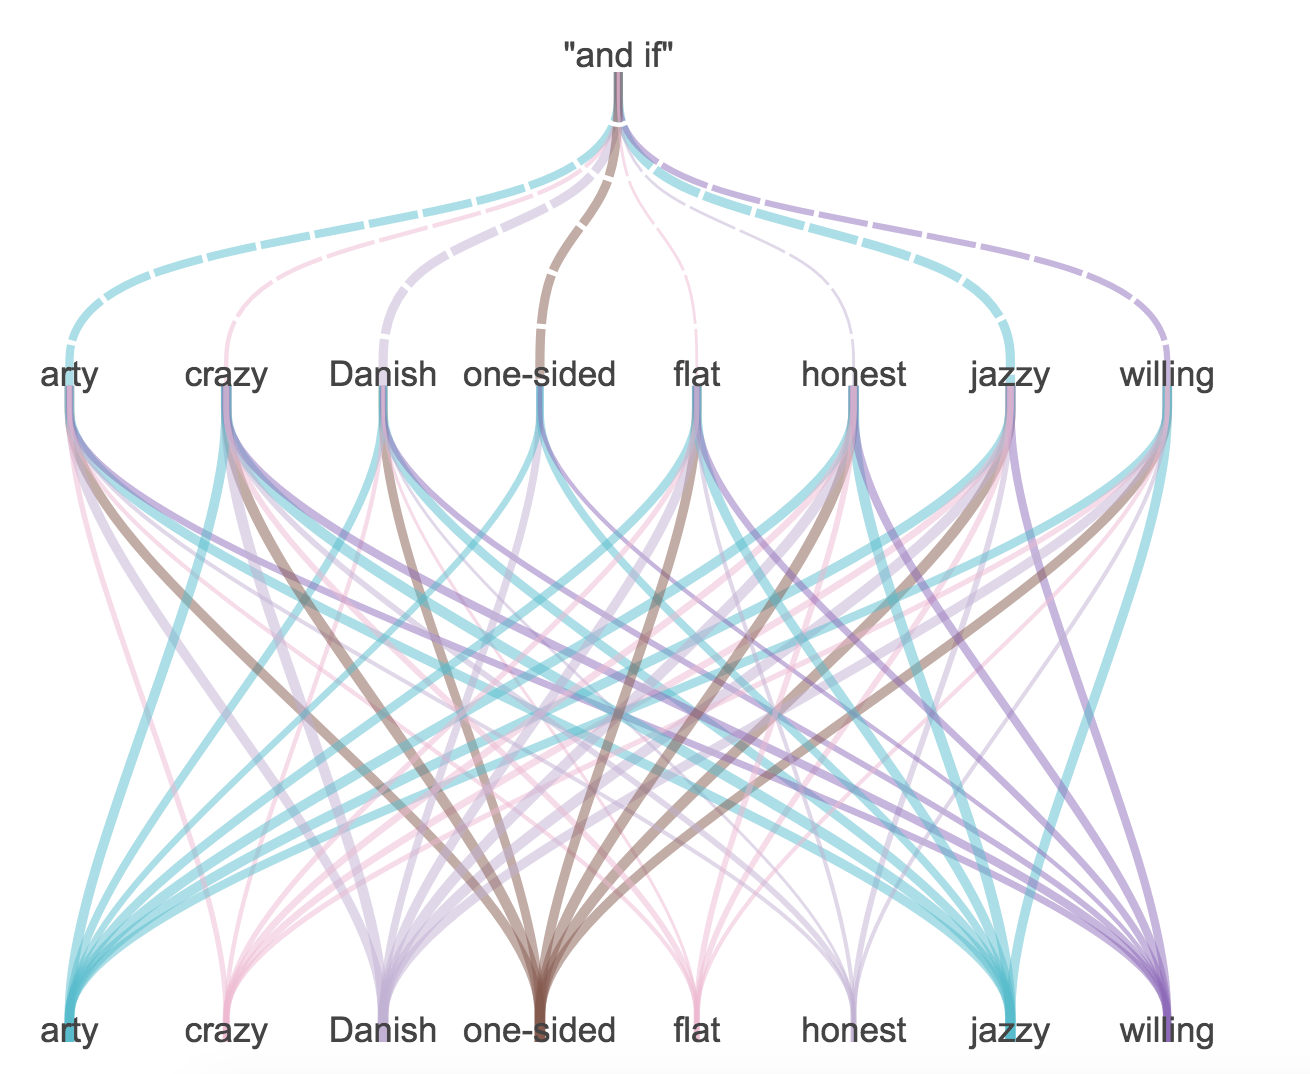
\includegraphics[width=16cm]{img/cooc_english2.png}
\caption{Main cooccurrences for \textit{and if} and \textit{fall} showed by Hyperbase}
\label{data_english}
\end{center}
\end{figure}


\subsection{Dataset : French}

The french data set is about political discourses. It's a corpus of 2.5 millions of words of French president from 1958 (with C. de Gaulle, the first president of the fifth republic) to 2018 with the first discourses of E. Macron. In this corpus we only remove the December 31 speech of E. Macron to use it as test data set. On this discourse E. Macron is mainly recognized by the deeplearning (The training task was to be able to predict the correct president). To achieve this task the deep learning seems to succeed to find really complex pattern specific to E. Macron. For example in this sequence :

\begin{quote}
\textit{[...] notre pays \textcolor{red}{\textbf{advienne à}} l'école pour nos enfants, au travail pour l' ensemble de \textcolor{red}{\textbf{nos concitoyens}} pour le climat pour le quotidien de chacune et chacun d' entre vous . \textcolor{red}{\textbf{Ces transformations profondes}} ont commencé et se \textcolor{red}{\textbf{poursuivront}} avec la même force le même rythme la même intensité [...]} 
\end{quote}

The Z-score brings statistically closer to De Gaulle than E. Macron. The error of statistical attribution can be explained by a Gaullist phraseology and the multiplication of linguistic markers strongly indexed by de Gaulle: for example, de Gaulle had the characteristic of making long and literary sentences articulated around conjunctions of coordination as \textit{et} (z-score = 28 for de Gaulle, 2 occurrences in the excerpt). His speech was also more conceptual than the average, and this resulted in an over-use of the articles defined \textit{le}, \textit{la}, \textit{l\'}, \textit{les}) very numerous in the extract (7 occurrences); especially in the feminine singular (\textit{la republique}, \textit{la liberté}, \textit{la nation}, \textit{la guerre}, etc., here we have \textit{la même force}, \textit{la même intensité}.

Les meilleures performances du deep learning interrogent quant à elle le linguiste et épouse parfaitement ce que l'on sait socio-linguistiquement du discours dynamique de Macron.

The most important activation zone of the extract concerns the nominal syntagm \textit{transformations profondes}. Taken separately, none of the two words of the phrase are very Macronian from a statistical point of view (\textit{transformations} = 1.9 \textit{profondes} = 2.9). Better: the syntagm itself is not attested in the corpus of learning of the President (0 occurrence). However, it can be seen that the co-occurrence of \textit{transformation} and \textit{profondes} amounts to 4.81 at Macron: so it is not the occurrence of one word alone, or the other, which is Macronian but the simultaneous appearance of both in the same window. The second and complementary activation zones of the extract thus concern the two verbs \textit{advienne} and \textit{poursuivront}. From a semantic point of view, the two verbs perfectly conspire, after the phrase \textit{transformations profondes}, to give the necessary dynamic to a discourse that advocates change. But it is the verb tenses (borne by the morphology of the verbs) that appear to be determining in the analysis. The calculation of the grammatical codes co-occurring with the word \textit{transformations} thus indicates that the verbs in the subjunctive and the verbs in the future (and also the nouns) are the privileged codes at Macron (Figure \ref{macron}). 

\begin{figure}[h]
\begin{center}
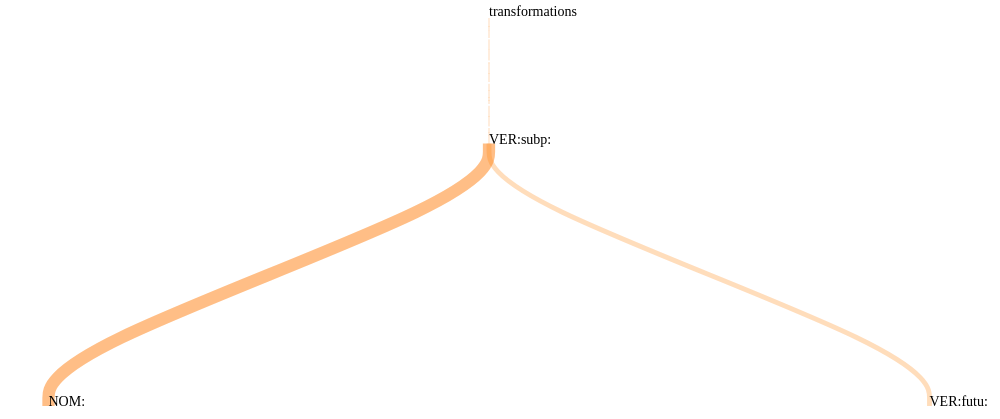
\includegraphics[width=10cm]{img/macron_cooc.png}
\caption{Main part-of-speech cooccurrences for \textit{transformations} showed by Hyperbase}
\label{macron}
\end{center}
\end{figure}


More precisely, the algorithm indicates that, in Macron, when \textit{transformation} is associated with a verb in the subjunctive (here \textit{advienne}), then there is usually a verb in the future co-present (here \textit{poursuivront}). \textit{transformations profondes}, \textit{advienne} to the subjunctive, \textit{poursuivront} to the future: all these elements sign, together, a speech made of promise of action, in the mouth of a young and dynamic president. Finally, the graph indicates that \textit{transformations} is especially associated with names in the President: in an extraordinary concentration, the extract lists 11 (\textit{pays}, \textit{école}, \textit{enfants}, \textit{travail}, \textit{concitoyens}, \textit{climat}, \textit{quotidien}, \textit{transformations}, \textit{force}, \textit{rythme}, \textit{intensité}).

\subsection{Dataset : Latin}

\begin{quote}
\textit{[...] tutus tenebat se quoad multum ac diu PAD quattuor milia peditum et quingenti equites in supplementum missi ex PAD sunt . tum refecta tandem spe \textcolor{red}{\textbf{castra propius hostem}} mouit classem que et ipse instrui parari que iubet ad insulas maritimam que oram tutandam . in \textcolor{red}{\textbf{ipso impetu}} mouendarum de [...]} 
\end{quote}

As historians, Caesar and Livy share a number of specific words:
- tool words, here (reflexive pronoun) -que (= "and", a coordinator), prepositions in "in", ad "to", ex "out of"
- names like equites "the riders" or "castra" the camp

The attribution of the sentence to Caesar can not rest on the specificities - that or in or castra, with differences equivalent or inferior to Livy. On the other hand, the differences of se, ex, are superior, as that of equites. Two very Caesarian terms undoubtedly make the difference iubet ("he orders") and ("milia" thousands).

The superior deviations of quattuor ("four"), "castra", "hostem" (the enemy), "impetu" ("the assault") at Titus Live are not enough to switch the attribution to this author .

On the other hand, the Deep Learning "activates" as "liviennes" several zones appearing at the beginning of sentence and corresponding to coherent syntactic structures:

- Tandem reflexes spe castra propius hostem mouit ": then the hope having finally returned, it approaches the camp closer to the camp of the enemy".

despite the fact that castra in hostem mouit is attested only by Tacitus

- in ipso metu: in fear itself ", while in X metu is attested 1x at Caesar and once at Quinte-Curce.

The hypothesis here is twofold:

- the structure tum + participates Ablative Absolute (tum refecta) is more characteristic of Titus Live (3.3, 8 occurrences) than of Caesar (1.7: 3 occurrences), even if it is even more specific of Tacitus (4 , 2: 10 occurrences).

- co-perpetratory castra and impetu networks may also have played a role:

impetu:
- in Titus Live, appear as cooccurrents lemmas HOSTIS 9.42 and CASTRA 6.75, while HOSTIS only has a gap of 3.41 in Caesar and that CASTRA does not appear in the list of cooccurrents impetu

castra:
the first cooccurent at Titus Live is HOSTIS (22,72), before CASTRA (10,18), AD (10,85), IN (8,21), IMPETVS (7,35), -QUE (5,86) )
while in Caesar, IMPETVS does not appear and the scores of all other lemmas are lower except CASTRA (15,15): HOSTIS (8),, AD (10,35), IN (5,17), - THAT (4.79)

